\chapter{腹部血管结构影像解剖}

腹部血管成像对于发现腹部病变的血供情况以及血管性病变有着十分重要的价值,因此需要我们能准确认识腹部的正常血管解剖结构。

\section{检查方法}

(一)MRA

MRA是目前应用较为广泛的一种无创血管成像方法之一,尤其它对于一些较为粗大的血管成像有较高的价值,比如主动脉及其主要的分支血管,腹部的大血管。据文献报道,目前较为成熟的MRA技术已经能够获得与DSA相同效果的图像。

对于每一例需进行腹部血管(包括腹腔动脉,肠系膜上下动脉,肾动脉,门静脉系统等)的MRA检查的患者都常规使用造影剂------马根维显45ml(3支)。首先先静脉推注造影剂20ml,然后再缓慢推注25ml造影剂与生理盐水30ml的混合液。在注药的同时启动扫描,并嘱咐患者屏气配合检查,最后在扫描结束后选择最佳的时相进行后重建,以获得腹部血管的三维图像,重建方式主要是MIP法。

扫描参数及技术:主要应用3D-FFE(快速梯度回波3D成像)序列进行动态扫描以获得重建的原始图像。该方法能利用流入性增强(inflow)效应获得较好的血管影像。扫描时所选的扫描方向为冠状面,扫描层厚为2mm,选用的矩阵为512×512。

(二)CTA

CTA技术是随着螺旋CT的出现,特别是多排螺旋CT(MSCT)较为广泛地应用后而快速发展起来的。目前的16排螺旋CT对于一些较为细小的血管,如颅内动脉及冠状动脉等都能较好地显示,并且能部分地替代传统的DSA造影。因此,对于腹部而言,较为粗大的腹部血管能通过CTA技术很好地显示。

对于每一例需进行腹部血管成像的患者均按体重适当使用非离子型碘造影剂,用量为1.5~2ml/kg。造影剂注射速度为3.5~4ml/s。

扫描技术:利用(smartprep)技术进行监测,当感兴趣区(一般为腹主动脉)的CT值到达预设值时自动触发扫描第一期------动脉期。然后延迟适当时间后进行静脉期扫描。为了减少每一次的扫描时间,每次扫描层厚为10mm,螺距为1.375∶1。扫描完成后,进行原始图像的薄层重建,重建图像层厚为2.5mm,间隔为1.5mm。

后处理技术:根据检查的目的,利用上述的薄层重建图像可以进行多种不同的重建,如获取VR(容积再现),MIP,VE(仿真内镜)的3D图像,亦可以进行MPR(多平面重建)的2D重建。

\section{断面血管影像}

轴位影像是我们阅读CT片的基础,因此有必要首先了解腹部血管的横断面影像解剖,以下是腹部主要血管的横断面影像。

\begin{figure}[!htbp]
 \centering
 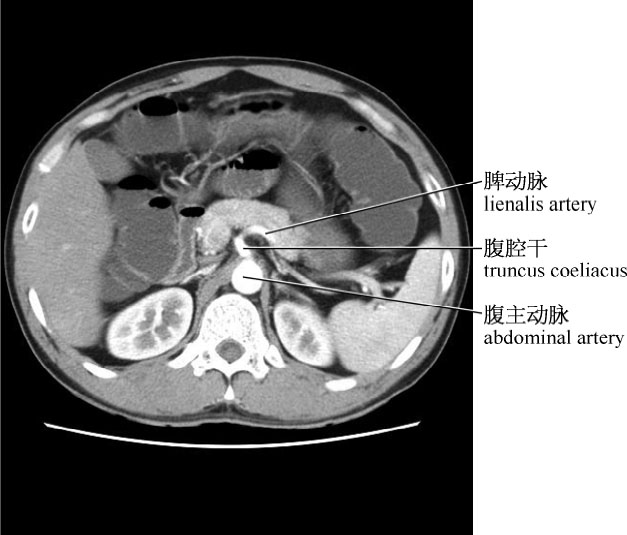
\includegraphics{./images/Image00191.jpg}
 \captionsetup{justification=centering}
 \caption{腹腔干}
  \end{figure} 
 \FloatBarrier

\begin{figure}[!htbp]
 \centering
 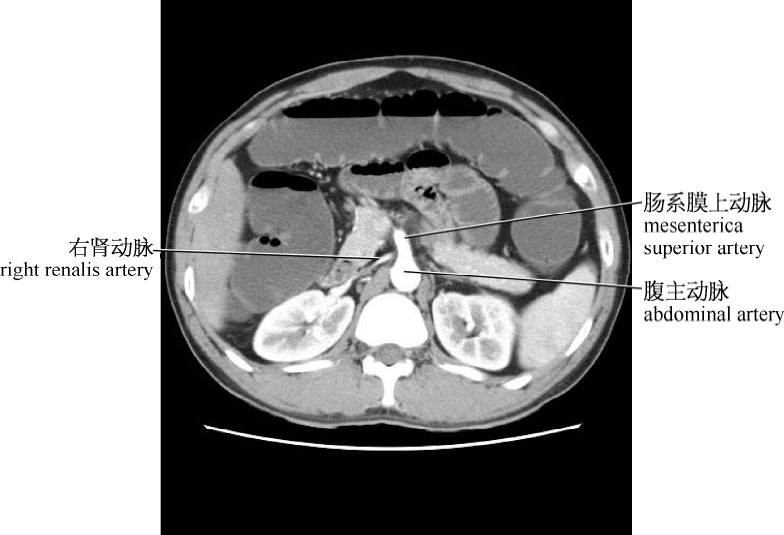
\includegraphics{./images/Image00192.jpg}
 \captionsetup{justification=centering}
 \caption{肠系膜上动脉}
  \end{figure} 
 \FloatBarrier

\begin{figure}[!htbp]
 \centering
 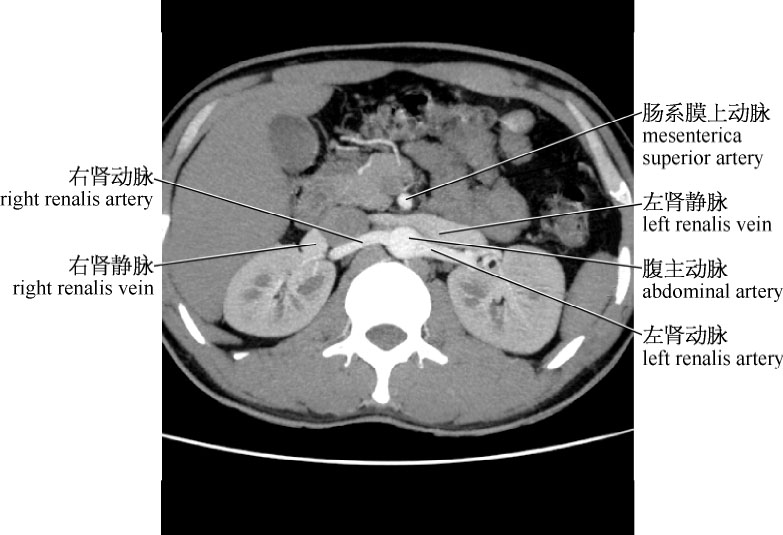
\includegraphics{./images/Image00193.jpg}
 \captionsetup{justification=centering}
 \caption{双肾动脉}
  \end{figure} 
 \FloatBarrier

\begin{figure}[!htbp]
 \centering
 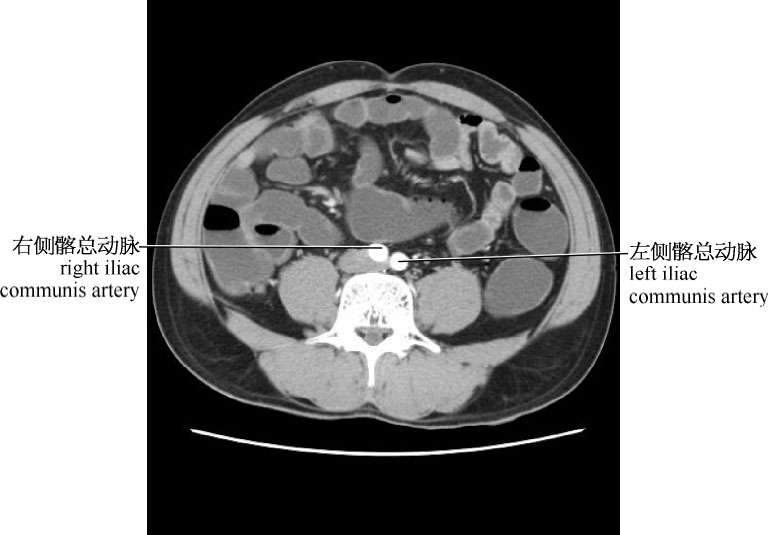
\includegraphics{./images/Image00194.jpg}
 \captionsetup{justification=centering}
 \caption{双侧髂总动脉}
  \end{figure} 
 \FloatBarrier

\begin{figure}[!htbp]
 \centering
 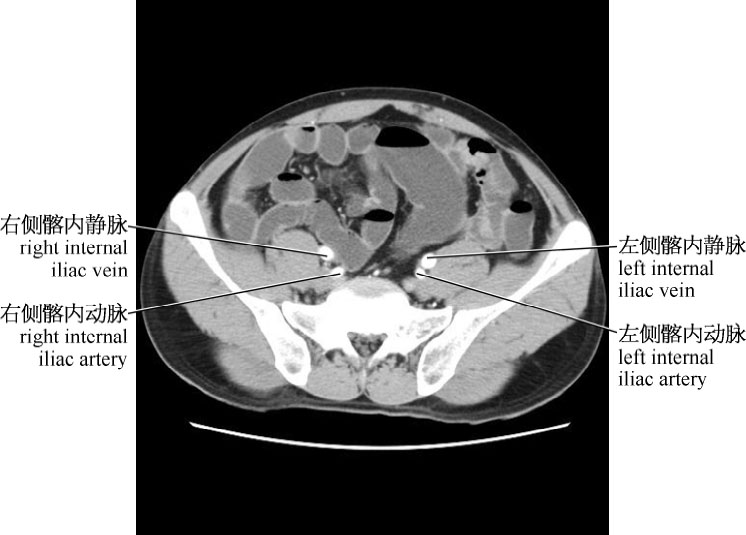
\includegraphics{./images/Image00195.jpg}
 \captionsetup{justification=centering}
 \caption{双侧髂内、外动静脉}
  \end{figure} 
 \FloatBarrier

因血管走行不同,故在冠状面时显示的主要是向左右走行的血管,如双侧肾动脉能显示较为理想。
\begin{figure}[!htbp]
 \centering
 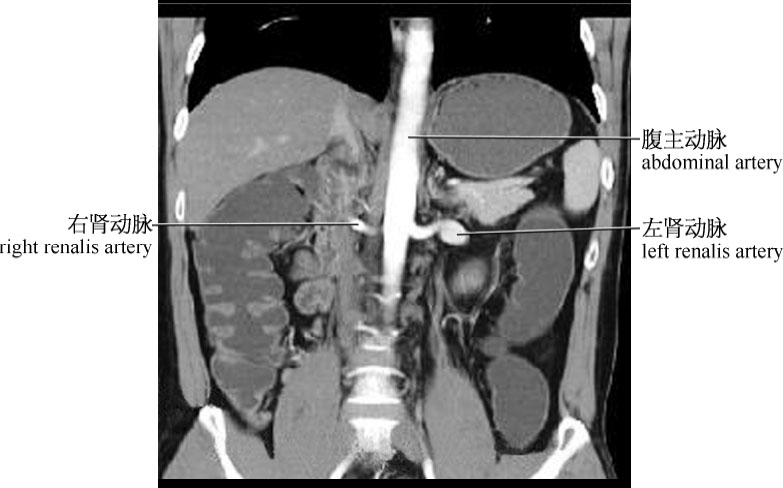
\includegraphics{./images/Image00196.jpg}
  \end{figure} 
 \FloatBarrier

\begin{figure}[!htbp]
 \centering
 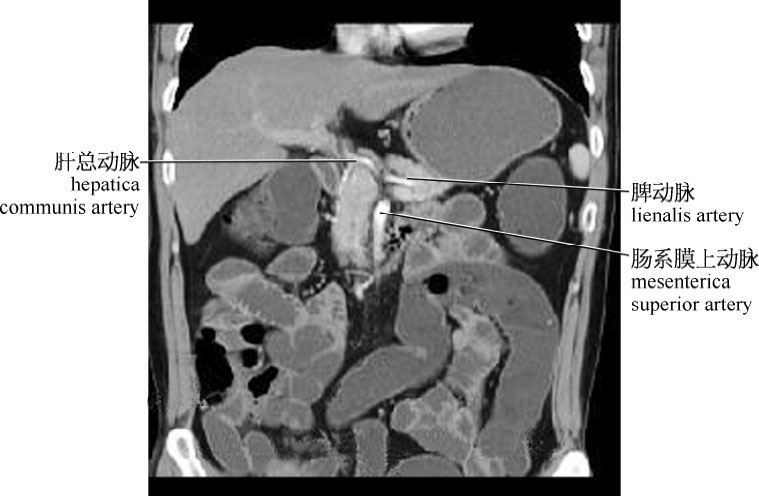
\includegraphics{./images/Image00197.jpg}
  \end{figure} 
 \FloatBarrier



在矢状面时显示的主要是向前后走行的血管,如肠系膜上动脉及腹腔动脉能显示较为理想。\begin{figure}[!htbp]
 \centering
 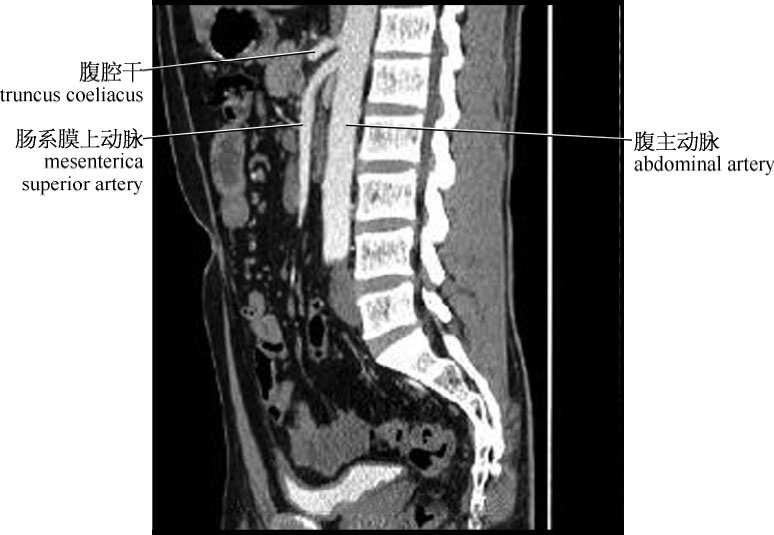
\includegraphics{./images/Image00198.jpg}
  \end{figure} 
 \FloatBarrier


\section{CTA和MRA血管解剖}

腹腔动脉------腹主动脉第一支主要分支血管,大约自T12至L1椎体间发出,一般血管开口指向前方。腹腔动脉常见有三个主要分支:肝总动脉,脾动脉,胃左动脉。

肠系膜上动脉------腹主动脉第二支主要分支血管,大约自L1椎体中部发出,一般血管开口指向前方偏右。

双侧肾动脉------腹主动脉第三对主要分支血管,大约自L1至L2椎体间发出,一般血管开口指向两侧,血管水平走行。

肠系膜下动脉------大约自L3椎体中部发出,一般血管开口指向前方偏左,通常血管较细。

双侧髂动脉------腹主动脉走行至L4椎体水平分叉形成。
\begin{figure}[!htbp]
 \centering
 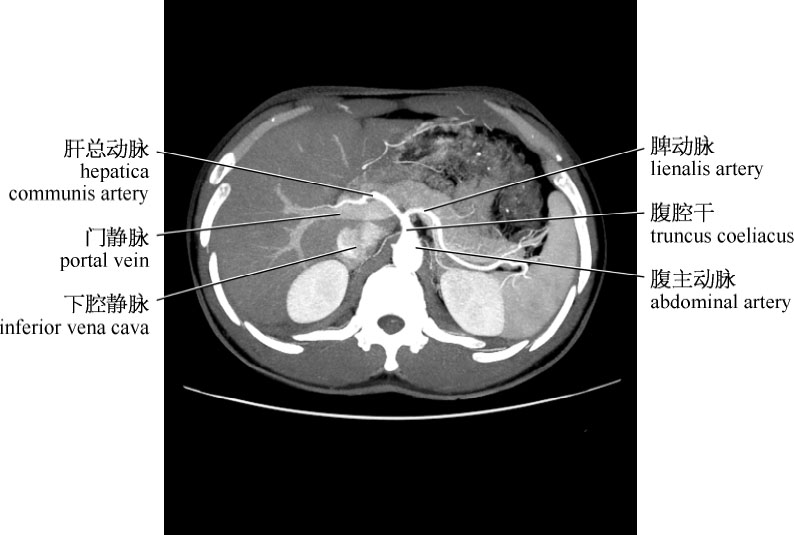
\includegraphics{./images/Image00199.jpg}
  \end{figure} 
 \FloatBarrier

\begin{figure}[!htbp]
 \centering
 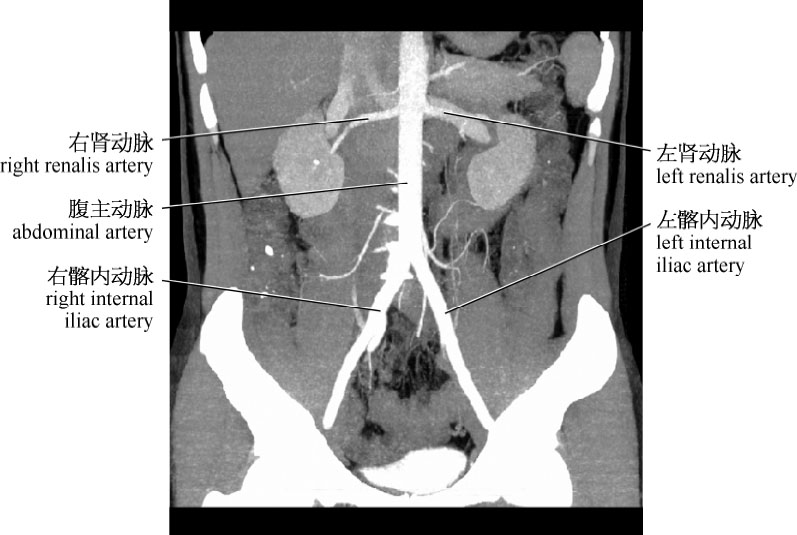
\includegraphics{./images/Image00200.jpg}
  \end{figure} 
 \FloatBarrier

\begin{figure}[!htbp]
 \centering
 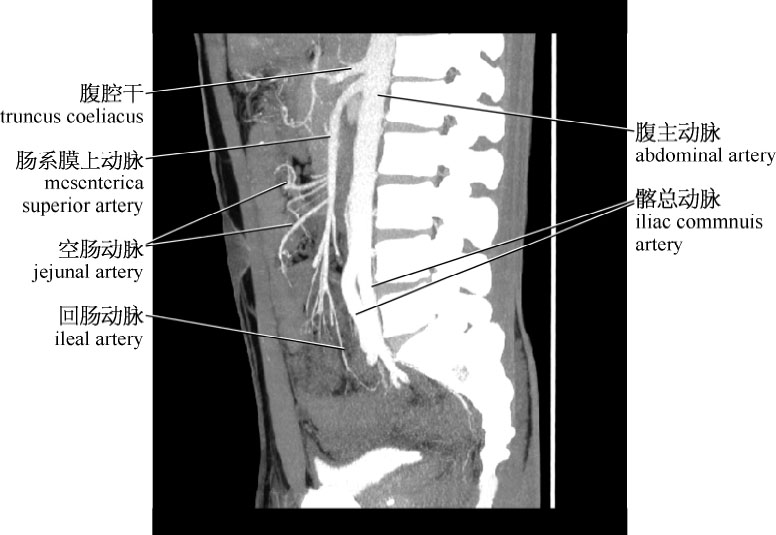
\includegraphics{./images/Image00201.jpg}
  \end{figure} 
 \FloatBarrier

\begin{figure}[!htbp]
 \centering
 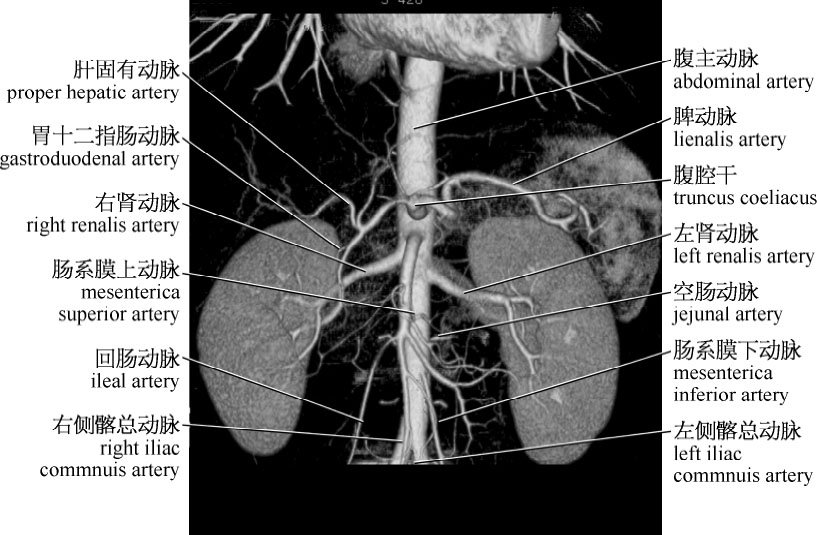
\includegraphics{./images/Image00202.jpg}
  \end{figure} 
 \FloatBarrier

\begin{figure}[!htbp]
 \centering
 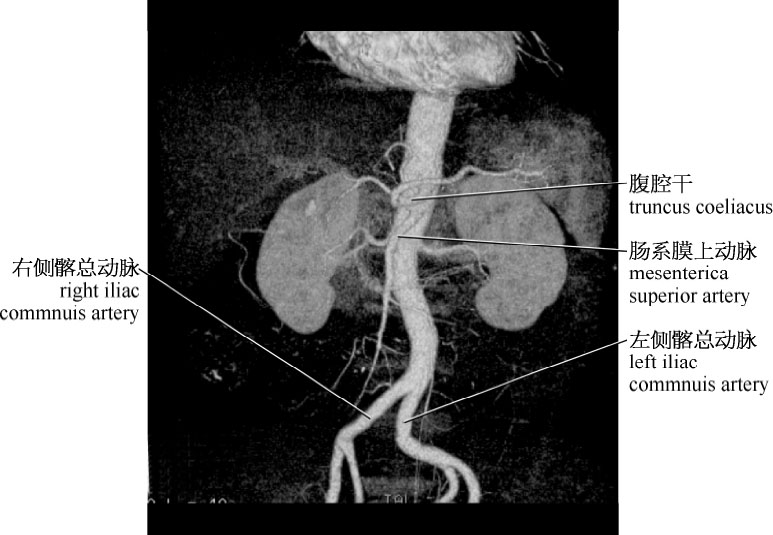
\includegraphics{./images/Image00203.jpg}
  \end{figure} 
 \FloatBarrier

